\documentclass[a4j,uplatex,dvipdfmx]{jsarticle}
\usepackage{amsmath}
\usepackage{tcolorbox}
\usepackage{graphicx}
\tcbuselibrary{breakable, skins, theorems}

\title{確率情報理論第19回}
\author{加藤まる}
\date{2020/03/19}

\begin{document}
\maketitle

\section*{本日の問題}
集合$A=\{ 1,2\}$と$B=\{ 1,2,3 \}$に対して、次の表に示す同時確率にしたがい$A \times B$の要素をとる確率変数(X,Y)を考える。
\begin{itemize}
  \item[(1)]エントロピーH(X)とH(Y)を求めよ。
  \item[(2)]同時エントロピーH(X,Y)を求めよ。
  \item[(3)]条件付きエントロピーH(X|Y)とH(Y|X)を求めよ。
  \item[(4)]相互情報量I(X;Y)を求めよ。   
\end{itemize}
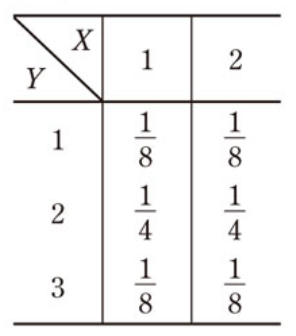
\includegraphics[width=5cm]{sec19fig.png}




解答を加藤まる(まるぼう)にDiscordDMに送ると添削します(添削不要の場合DMは不要)。解答は夜にDiscordに貼るので自己採点してみてください。

\end{document}